\documentclass[11pt,oneside,letterpaper]{article}

% graphicx package, useful for including eps and pdf graphics
\usepackage{graphicx}
\DeclareGraphicsExtensions{.pdf,.png,.jpg}

% basic packages
\usepackage{color} 
\usepackage{parskip}
\usepackage{float}

% text layout
\usepackage{geometry}
\geometry{textwidth=15cm} % 15.25cm for single-space, 16.25cm for double-space
\geometry{textheight=22cm} % 22cm for single-space, 22.5cm for double-space

% helps to keep figures from being orphaned on a page by themselves
\renewcommand{\topfraction}{0.85}
\renewcommand{\textfraction}{0.1}

% bold the 'Figure #' in the caption and separate it with a period
% Captions will be left justified
\usepackage[labelfont=bf,labelsep=period,font=small]{caption}

% review layout with double-spacing
%\usepackage{setspace} 
%\doublespacing
%\captionsetup{labelfont=bf,labelsep=period,font=doublespacing}

% cite package, to clean up citations in the main text. Do not remove.
\usepackage{cite}
%\renewcommand\citeleft{(}
%\renewcommand\citeright{)}
%\renewcommand\citeform[1]{\textsl{#1}}

% Remove brackets from numbering in list of References
\renewcommand\refname{\large References}
\makeatletter
\renewcommand{\@biblabel}[1]{\quad#1.}
\makeatother

\usepackage{authblk}
\renewcommand\Authands{ \& }
\renewcommand\Authfont{\normalsize \bf}
\renewcommand\Affilfont{\small \normalfont}
\makeatletter
\renewcommand\AB@affilsepx{, \protect\Affilfont}
\makeatother

% comments
\usepackage{ulem}
\definecolor{purple}{rgb}{0.459,0.109,0.538}
\def\tb#1#2{\sout{#1} \textcolor{purple}{#2}} 
\def\tbc#1{\textcolor{purple}{[#1]}}

\begin{document}

\section*{Linkage disequilibrium data}

\begin{figure}[h]
\centering  
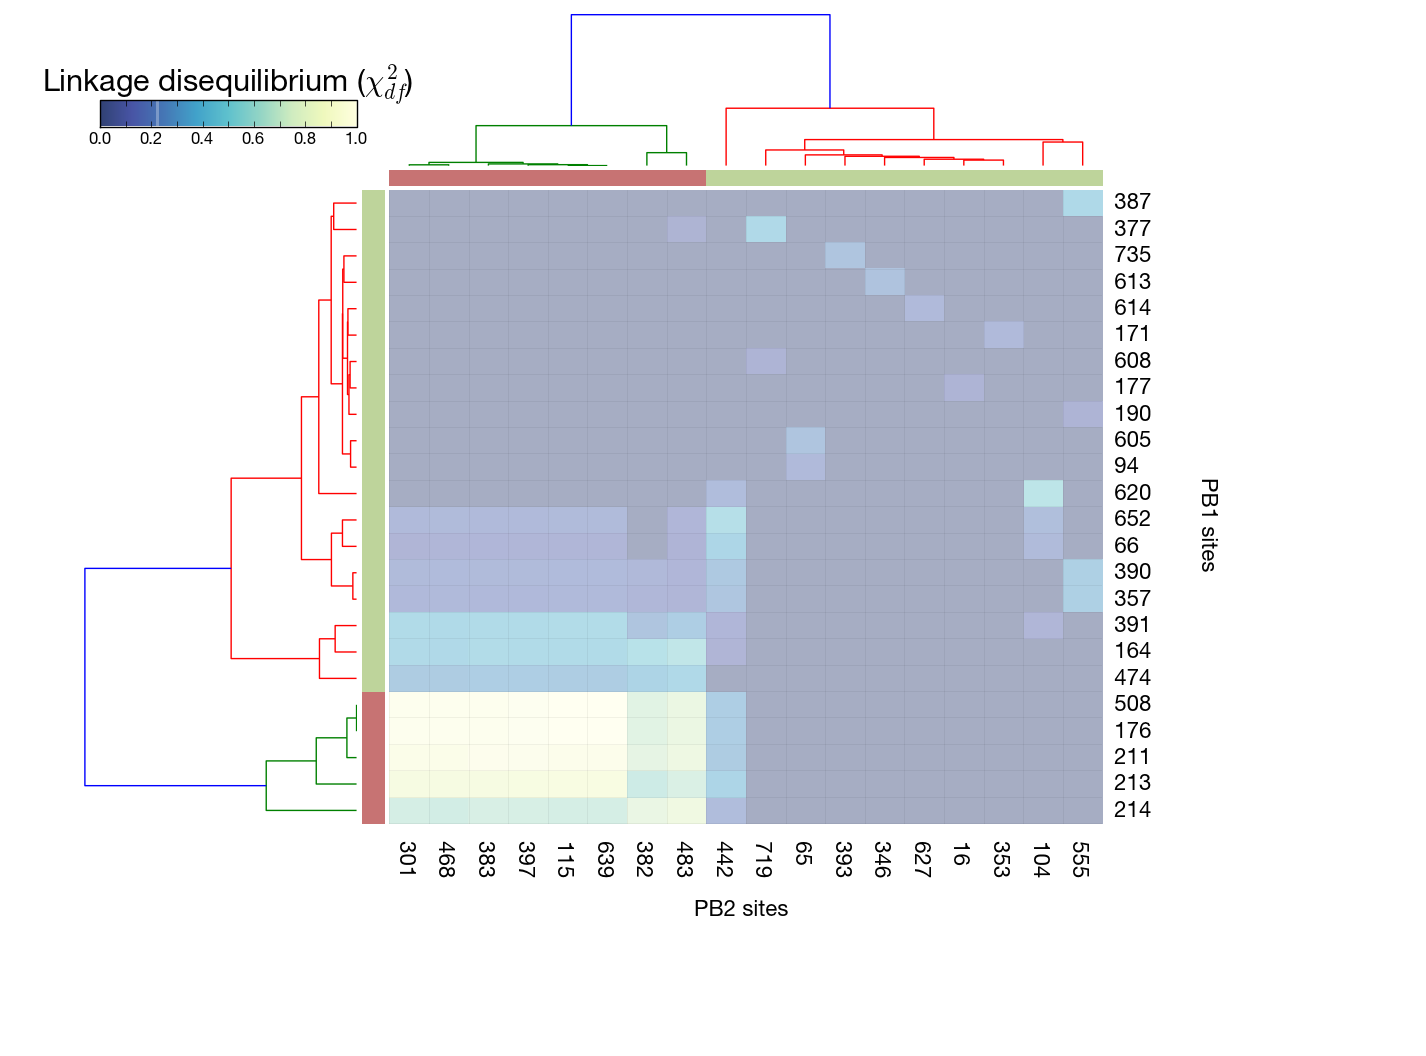
\includegraphics[width=0.65\textwidth]  {supp_figures/Chi_PB1_PB2.png}
\caption{\textbf{Hierarchical clustering of amino acid sites on PB1 and PB2 segments based on $\chi^{2}_{df}$ values.}}
\label{ChiPB1PB2}
\end{figure}


\begin{figure}[h]
\centering  
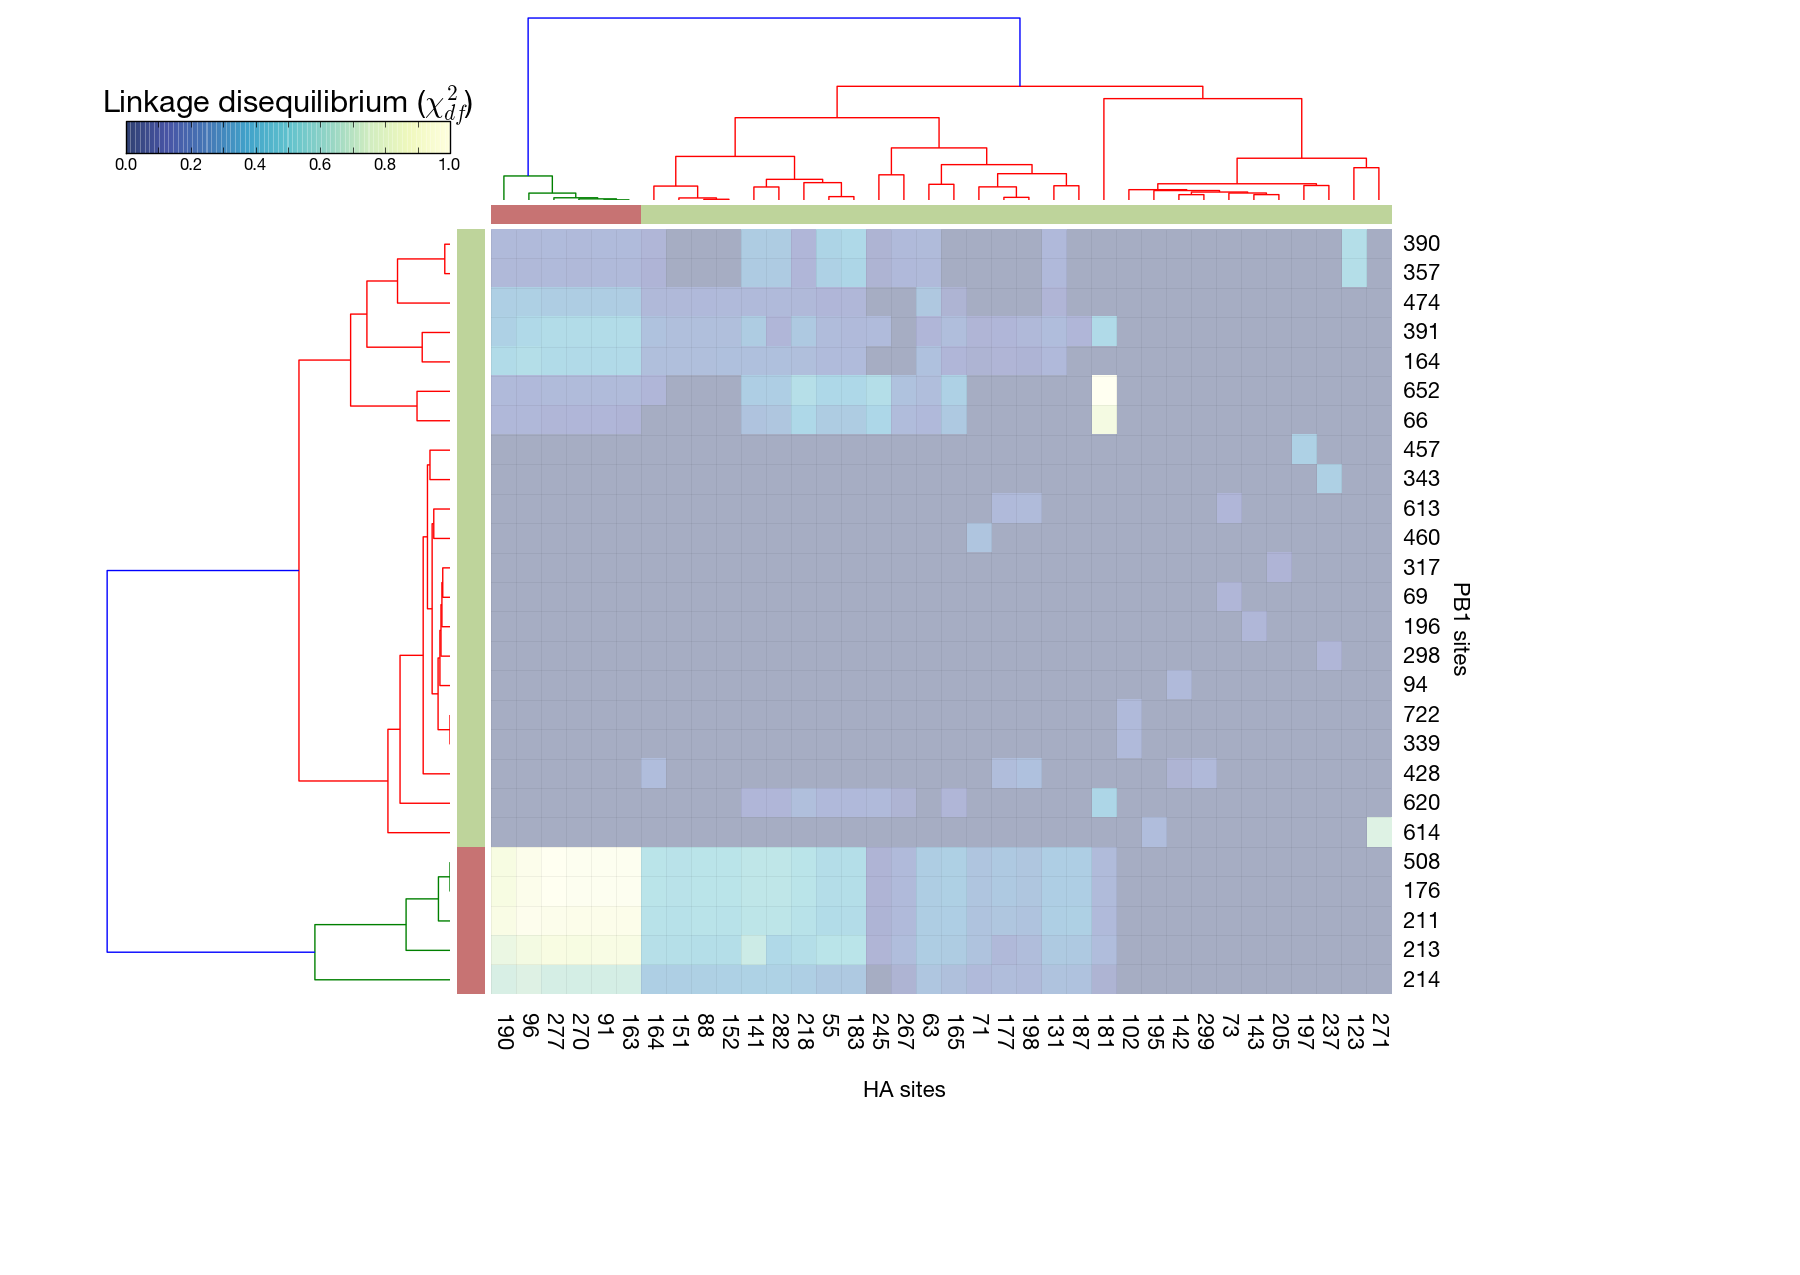
\includegraphics[width=0.65\textwidth]  {supp_figures/Chi_PB1_HA.png}
\caption{\textbf{Hierarchical clustering of amino acid sites on PB1 and HA segments based on $\chi^{2}_{df}$ values.}}
\label{ChiPB1HA}
\end{figure}


\begin{figure}[h]
\centering  
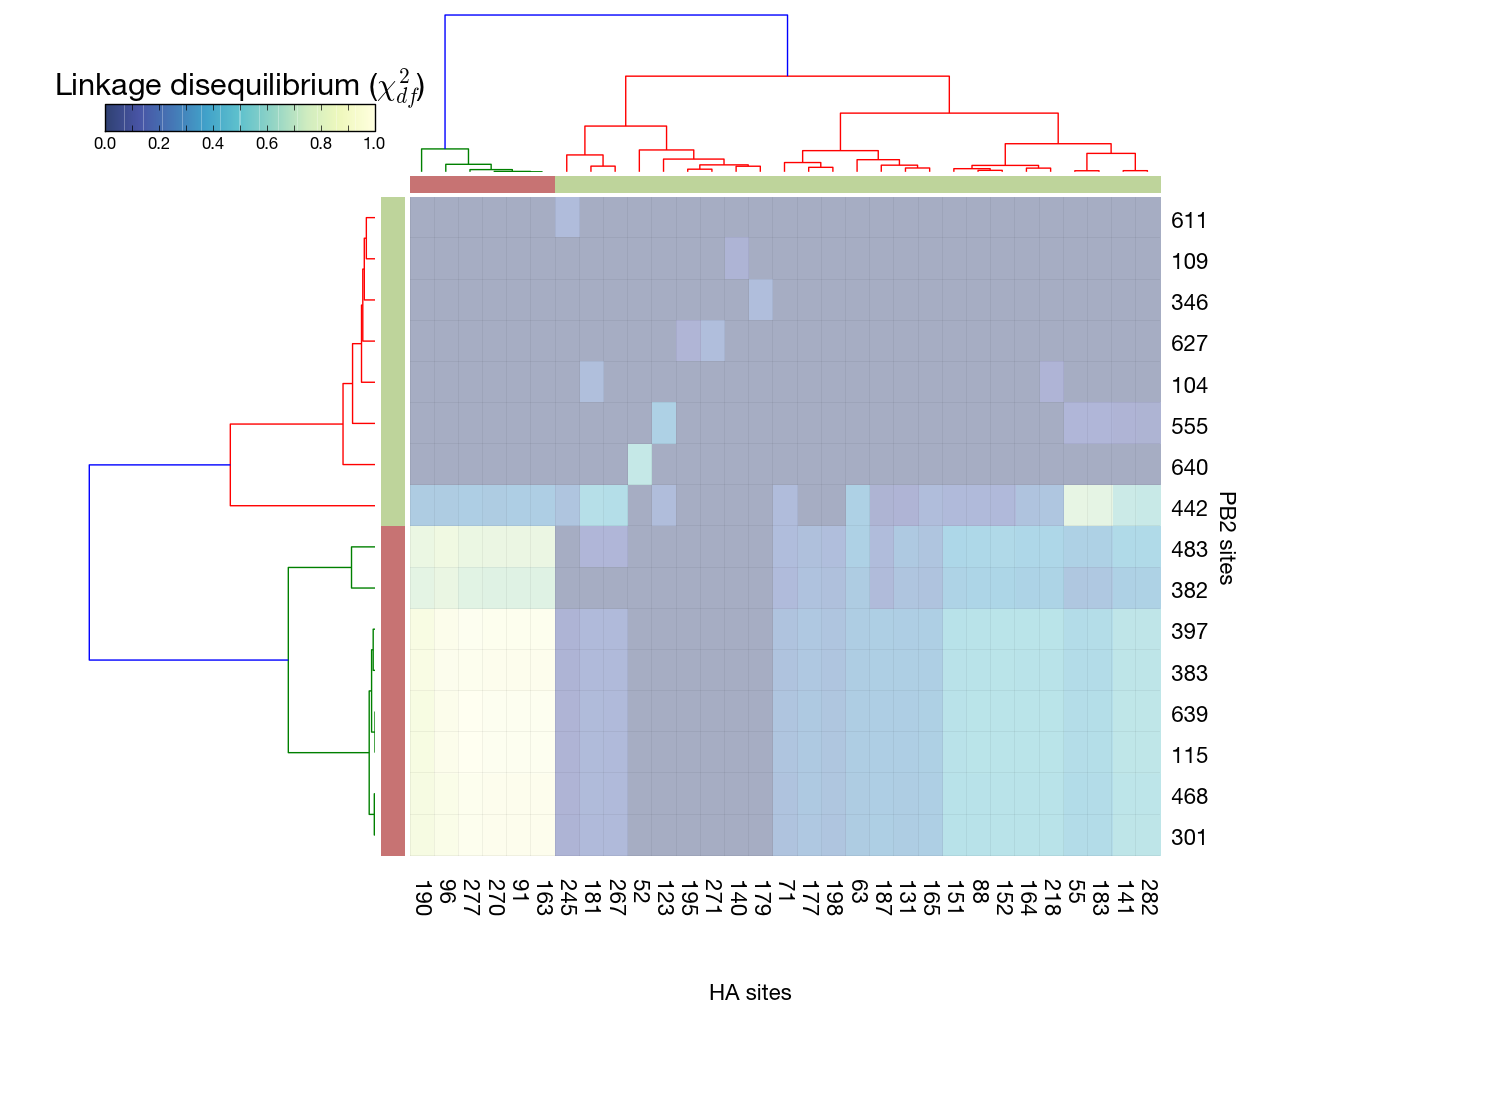
\includegraphics[width=0.65\textwidth]  {supp_figures/Chi_PB2_HA.png}
\caption{\textbf{Hierarchical clustering of amino acid sites on PB2 and HA segments based on $\chi^{2}_{df}$ values.}}
\label{ChiPB2HA}
\end{figure}

We have identified amino acid sites which exhibit a high degree of linkage disequilibrium between PB1, PB2 and HA segments.
Sites with high LD on PB1, PB2 and HA segments could be interpreted as either sites which have drifted apart due to lack of reassortment between the three segments or as sites which prevent the cooperation of the three proteins at the molecular level and thus prevent inter-lineage PB1-PB2-HA reassortants from having comparable fitness to viruses with `pure' lineage PB1-PB2-HA complexes.

None of the sites we have identified on PB1 and PB2 proteins fall within the previously described regions that form the contacts between the two polymerase subunits \cite{sugiyama2009}.

Sites 211, 213 and 214 on the PB1 protein are very close to each other and the stretch of sequence around these residues contains many positively charged amino acids (lysine and arginine).
Multiple nuclear localization signals (NLSs) are predicted to occur around this region and sites 211, 213 and 214 are either predicted to be near the end of a mono-partite NLS or the beginning of a bi-partite NLS.
Previous research \cite{nath1990} suggests that in the influenza A PB1 protein residue 211 (homologous to influenza B PB1 residue 211) is the last residue of a bi-partite NLS.
Almost all Yamagata lineage isolates possess arginine (R) residue at PB1 positions 211 and 214 and a serine (S) residue at position 213, whereas Victoria lineage isolates have lysine (K) at positions 211 and 214 and threonine (T) at position 213.
It remains to be seen whether these sites significantly affect the nuclear import efficiency of the PB1 protein of either lineage.
Though the PB1 protein is known to accumulate in the nucleus on its own, efficient import into the nucleus requires the presence of the PA protein \cite{fodor2004}.
Similarly, sites 382 and 397 on the PB2 protein are close to residues 377, 406 and 408 which are homologous to sites in influenza A that are responsible for mRNA cap-binding \cite{guilligay2008}.
Again, we cannot determine whether this finding is significant or not.


\begin{figure}[h]
\centering  
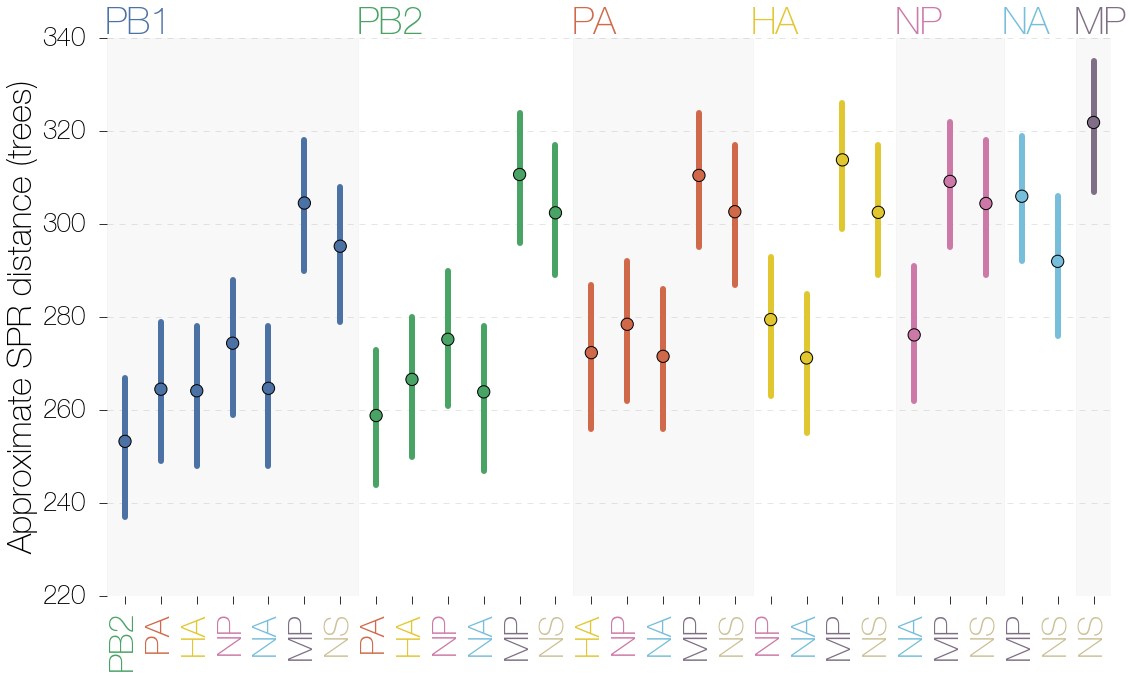
\includegraphics[width=0.65\textwidth]  {supp_figures/InfB_supp_aSPRdistances_trees.png}
\caption{\textbf{}}
\label{}
\end{figure}

\begin{figure}[h]
\centering  
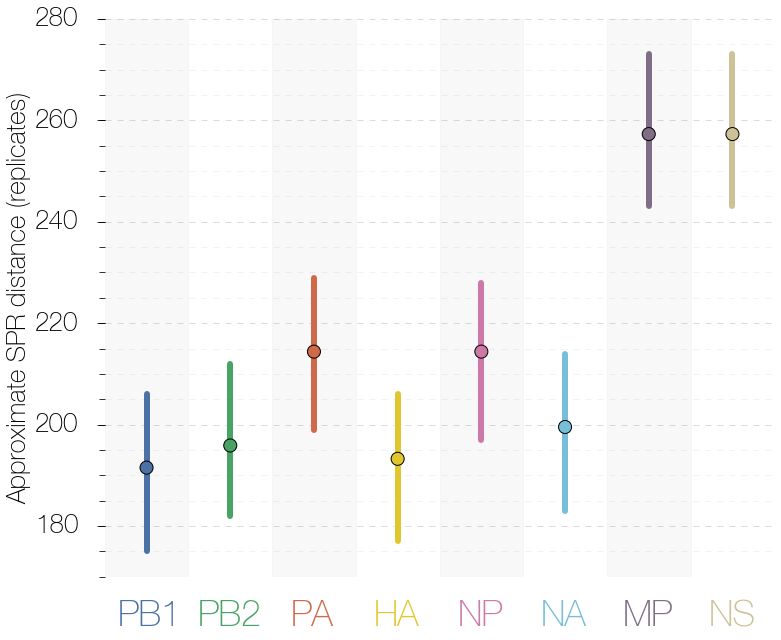
\includegraphics[width=0.65\textwidth]  {supp_figures/InfB_supp_aSPRdistances_replicates.png}
\caption{\textbf{}}
\label{}
\end{figure}

\begin{figure}[h]
\centering  
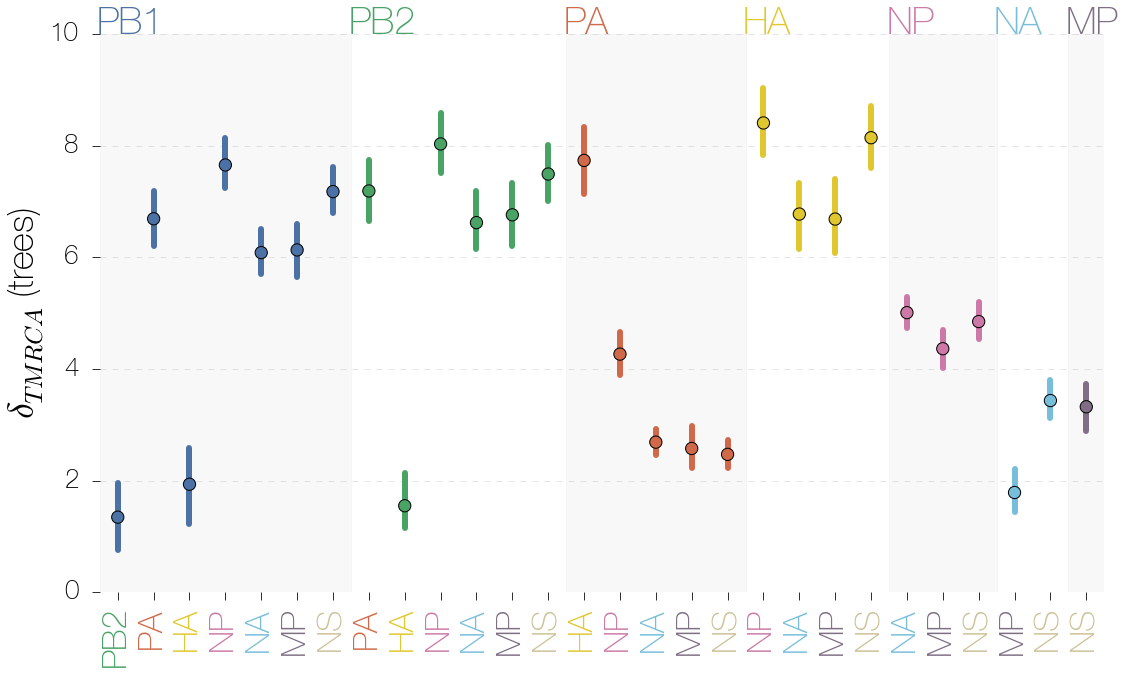
\includegraphics[width=0.65\textwidth]  {supp_figures/InfB_supp_deltaTMRCA_trees.png}
\caption{\textbf{}}
\label{}
\end{figure}

\begin{figure}[h]
\centering  
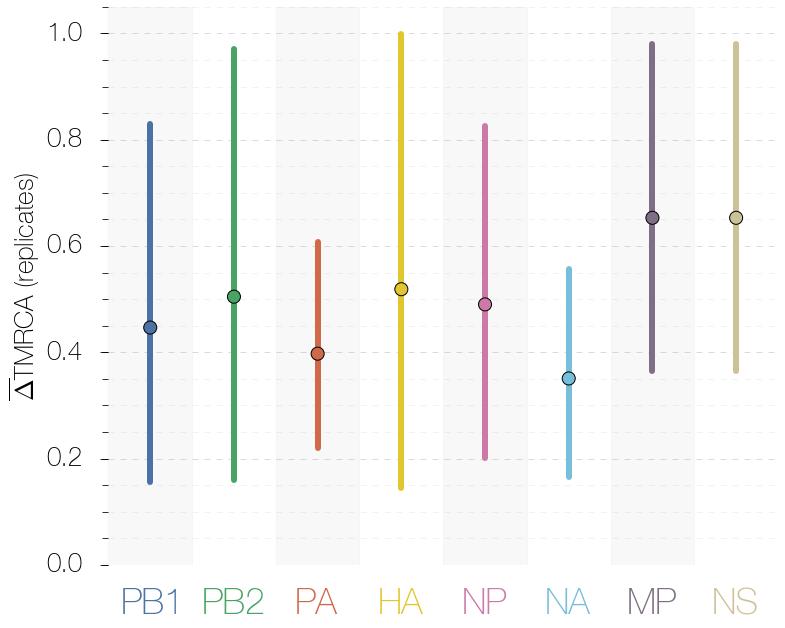
\includegraphics[width=0.65\textwidth]  {supp_figures/InfB_supp_deltaTMRCA_replicates.png}
\caption{\textbf{}}
\label{}
\end{figure}

\begin{figure}[h]
\centering  
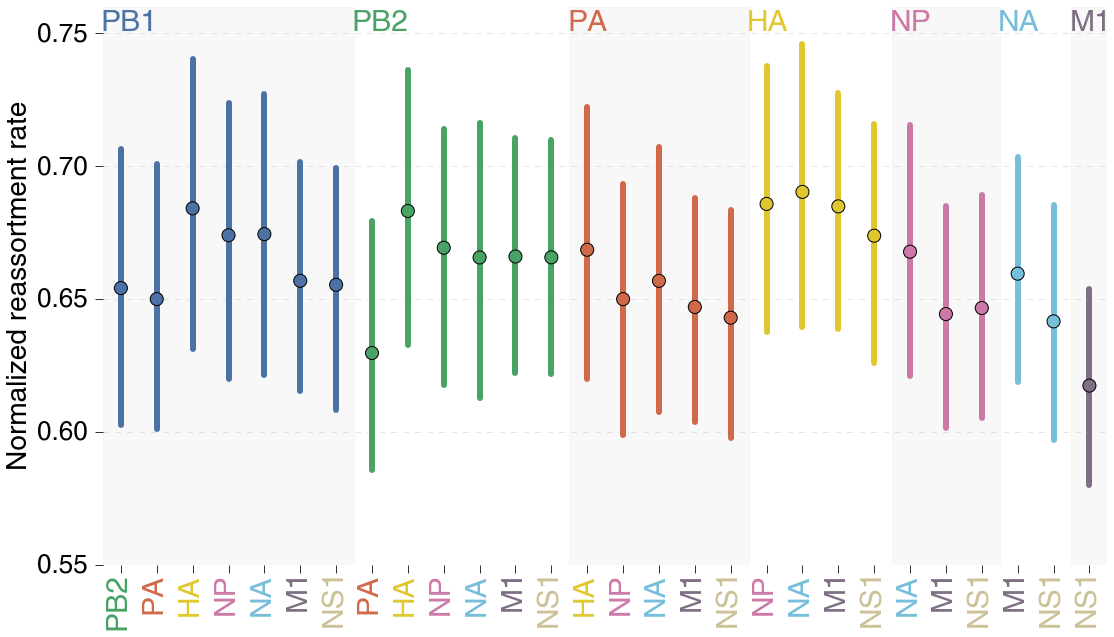
\includegraphics[width=0.65\textwidth]  {supp_figures/InfB_supp_normRErate.png}
\caption{\textbf{}}
\label{}
\end{figure}

\begin{figure}[h]
\centering  
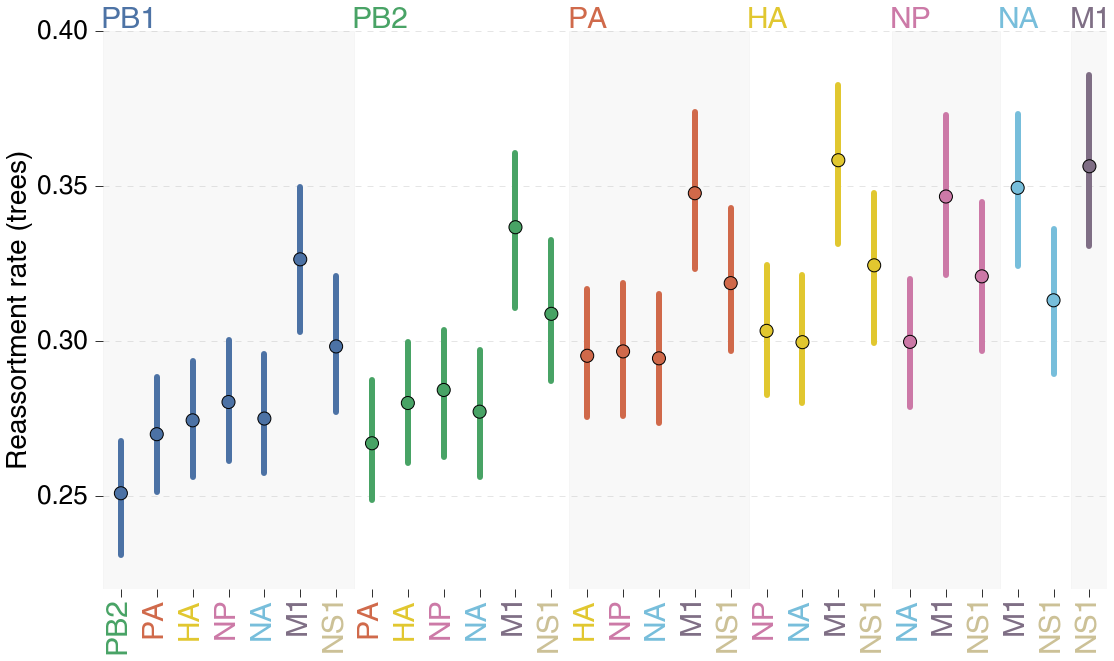
\includegraphics[width=0.65\textwidth]  {supp_figures/InfB_supp_RErate_trees.png}
\caption{\textbf{}}
\label{}
\end{figure}

\begin{figure}[h]
\centering  
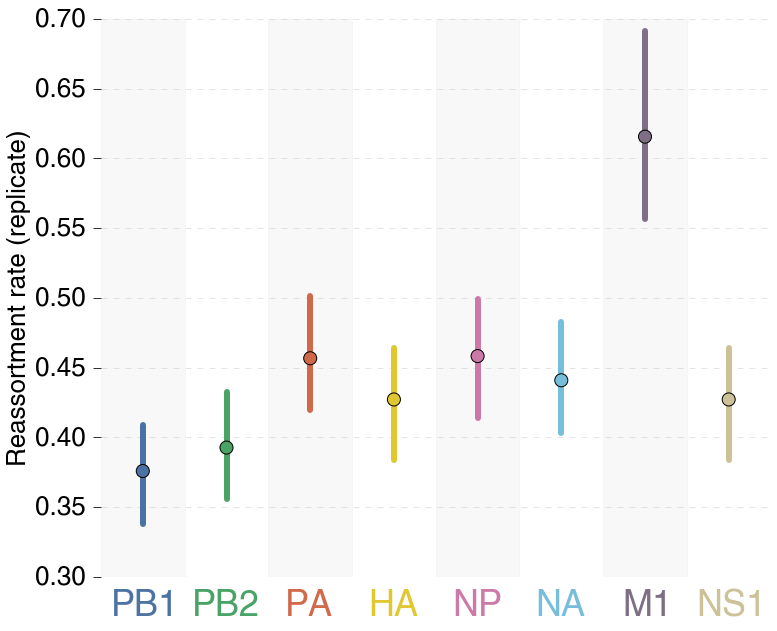
\includegraphics[width=0.65\textwidth]  {supp_figures/InfB_supp_RErate_replicates.png}
\caption{\textbf{}}
\label{}
\end{figure}


\bibliographystyle{pnas}
\bibliography{fluB}
\end{document}
